\documentclass{article}
\usepackage{graphicx}

\begin{document}
\title{Requirements Specification Document}
\author{Team D}
\date{\today}

\maketitle

\vspace*{1.5in}
\begin{table}[htbp]
\caption{Team}
\begin{center}
\begin{tabular}{|r | c|}
\hline
Name & ID Number \\
\hline\hline
Stefanie Lavoie & 1951750 \\
Pinsonn Laverdure & 9684352 \\
Ghislain Ledoux & 6376320 \\
Rigil Malubay & 6262732 \\
Philippe Milot & 9164111 \\
Christopher Mukherjee & 6291929 \\
\hline
\end{tabular}
\end{center}
\end{table}

\clearpage

\section{Introduction} % Status: COMPLETE

This document will describe in detail the requirement specifications for the Vessel Monitoring System which is to be developped in the context of the COMP354 course. The requirements specifications include an overview of the system and its goals, a detailed description of all functional and non-functional requirements (modelled using Use Case Diagrams and Domain Model Diagrams), as well as a development plan. 

If a requirement appears in this document, the final Vessel Monitoring System \emph{must} conform to this requirement. Inversely, the Vessel Monitoring System is not requirement to conform to any other requirement that is not specified in this document.

\section{Project Description} % Status: COMPLETE

The Vessel Monitoring System is a Java-based system which listens to incoming radar data from multiple vessels at sea and keeps track of their type, position, and velocity. The goal of the system is to ensure that no vessel ever collide with one another.

To accomplish this, the system tracks ``risk zones'' around each tracked vessel. The \emph{Low-Risk Zone} is defined as the circle area with a 200m radius around the vessel. The \emph{High-Risk Zone} is defined as the circle area with a 50m radius around the vessel. The system shall generate appropriate alarms when a dangerous situation arises, e.g. when two vessels's risk zones start to overlap. The system shall issue a \emph{Low-Risk Alert} whenever two or more Low-Risk Zones overlap. The system shall issue a \emph{High-Risk Alert} whenever two or more High-Risk Zones overlap.

The VMS has a graphical desktop application component. Radar data is visually accessible at all time in two different modes:

The \emph{List Mode} presents a list of all currently-tracked ships. Each row in the list contains all known metadata associated with a single ship: The Vessel ID, the Type, the X-Y coordinates, the Speed (in m/s), the Course, the Distance from starting point, and the time and date of last-received data. The list can be sorted by any of its columns, in both ascending and descending orders.

In this mode, the alerts are represented by highlighting the rows of the vessels involved in the alert. A Low-Risk Alert will highlight the rows in yellow. A High-Risk Alert will highlight the rows in red.

\begin{figure}[h]
\caption{A sketch of the user interface}
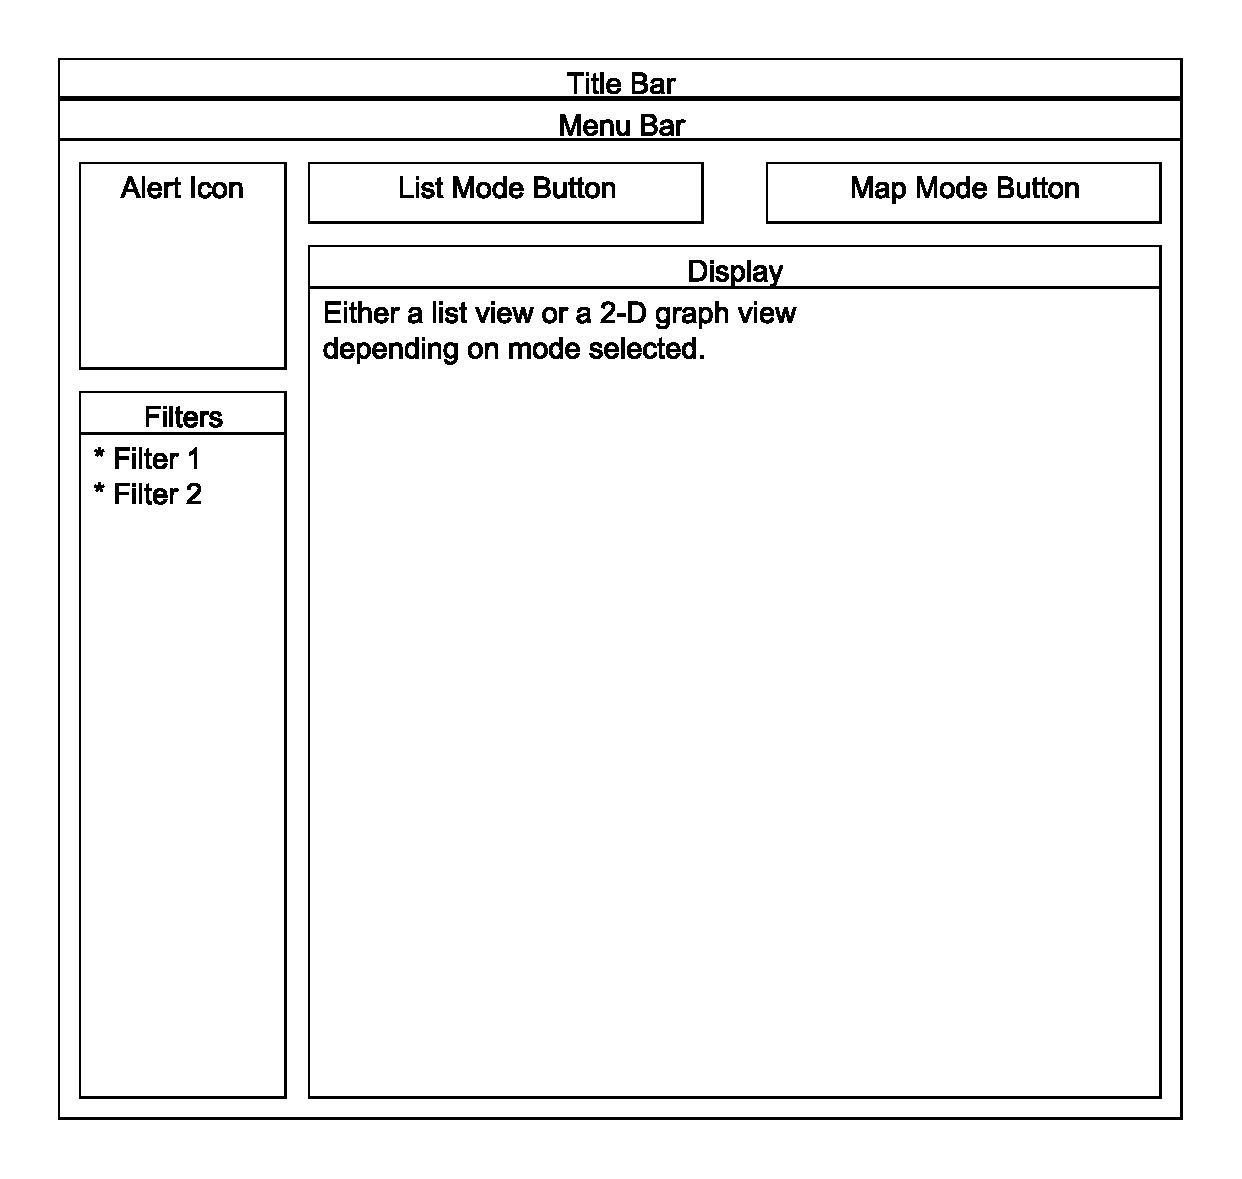
\includegraphics[width=\linewidth]{gui-proto.eps}
\end{figure}

The \emph{Map Mode} displays a 2-D grid where each tracked vessel is represented as a dot placed on the grid according to its X-Y coordinates. The colour of the dot represents the Vessel Type. Additionally, two wider circles around each dot represent the vessel's two ``risk zones''. The Low-Risk zone is displayed as an yellow circle. The High-Risk zone is displayed as a red circle.

In this mode, the alerts are represented by blinking the vessels involved in the alert. Since the zones are constantly represented visually, the type of alert is visible from simply looking at the grid.

Both view modes update the display in real-time, at a refresh rate which is configurable by the user. Both views can be filtered by Vessel Type. Both views display an ``Alert Icon'' in the top-left corner of the window. This icon is a large, white number against a colored background. The number represents how many alerts are currently in effect. The background color represents the severity of the highest-risk alert currently in effect (red for High-Risk, yellow for Low-Risk, green when no alerts are in effect).

\subsection{Vessel Simulator}

For the sake of testing, the system will also include a \emph{Vessel Simulator} which will emulate the behavior of a real vessel. The Simulator is a simple command-line utility which will read vessel data from a file, connect to the VMS, and periodically send updated vessel data to the VMS.

The format of the file is that of a standard VSF file. The description of the format is beyond the scope of this document.

\section{Goals and Constraints} % Status: See subsections.

\subsection{Functional Requirements} % Status: Need to incorporate UCDs from Stefanie and Pinsson.

\subsection{Domain Model} % Status: Need to create domain model diagram.

\subsection{Constraints} % Status: Satisfactory, but can keep adding as they are thought up.

\subsubsection{Shared constraints}
Both applications shall run on Windows 7 or later, and Mac OS X 10.8 or later.

Both applications shall require the Java 7 platform to run.

\subsubsection{VMS constraints}
Functionally, the VMS shall be limited to keeping track of 100 unique ships at any time. This is to avoid slowdown as the number of ships increase. If new data comes in that pushes the number of unique ships over that limit, the VMS shall ``forget'' the oldest ship already tracked to make room for the new one, and issue a warning to the human operator.

\subsubsection{Simulator constraints}

No user interface shall be designed for the Simulator. It is strictly a separate command-line tool.

Reading a timestep of less than 0.5 in the VSF file shall issue a parsing error, causing the program to exit immediately.

\section{Resource Evaluation} % Status: See subsections.

\subsection{Human Resources} % Status: Need Pinsson's description. Add availabilities.

\emph{Pinsson Laverdure} TBD.

\emph{Stefanie Lavoie} has experience with developping on the Java platform (but not using the Swing library for GUI), as well as managing a project's source code using the Git DVCS. Although she has never used \LaTeX before, she will be able to contribute significantly to the design and code of the project.

\emph{Ghislain Ledoux} has a good conciliatory nature which lends itself well to working in teams. He has a good instinct for identifying use cases, which will be useful in the first stages of design. He has no prior experience working with a source control system nor with \LaTeX.

\emph{Rigil Malubay} has good analytical and problem-solving skills. He has prior work experience as a web developer in PHP. According to himself, he lacks attention to detail, but this weakness is mitigated when working closely in a team.

\emph{Philippe Milot} has previous work experience with developping on a wide range of platforms and programming languages (C/C++, Java, Haskell, Perl, Python, PHP, \LaTeX, etc.), which will be useful for informing the technological choices that will be made for the project. He is familiar with Subversion and Git VCS. He has never worked with a Java GUI toolkit before.

\emph{Christopher Mukherjee} has experience with the Java platform as well as web programming. He has previous work experience with tech companies such as Trendex Information Systems and Ericsson. His experience with working in larger teams will help the project reach its deadlines on time. He has never worked with \LaTeX before.

\subsection{Technical Resources} % Status: COMPLETE

The project can make use of the software that is available in the computer labs of Concordia University. 

The project shall be developped in parallel on both Windows and Mac OS X platforms. Development can be done either on Concordia University's computers or the personal computers of the developers.

The project shall be developped on the Java platform version 7. All graphical user interfaces shall use the Swing library.

The project shall use Git as its source-control solution. GitHub shall be used for hosting the repository online.

The project shall use \LaTeX for typesetting all its documentation. Visio and UMLet shall be the tools used to create diagrams.

\section{Scoping} % Status: COMPLETE
The VMS shall not use a separate client/server architecture. The ``server'' part will be directly integrated into the desktop application. The Simulator (and other theoretical vessels) will have to connect to the desktop application to send their data.

Connection issues between the VMS and vessels shall be handled in the most basic way possible (display error message and exit).

No UI shall be provided to customize the limit of a 100 unique ships. Instead, the limit shall be configurable via a command-line argument when starting the VMS. 

No UI shall be provided to customize the address at which the VMS will listen to incoming data. Instead, the limit shall be configurable via a command-line argument when starting the VMS.

\section{Plan} % Status: To be done

\subsection{Activities}

\subsection{Project Estimates}

\subsection{Activities Assignments}

\subsection{Schedule}

\subsection{Risk}

\end{document}
